\documentclass{article}

% if you need to pass options to natbib, use, e.g.:
     \PassOptionsToPackage{square,numbers}{natbib}
% before loading neurips_2021

% ready for submission
%\usepackage{neurips_2021}

% to compile a preprint version, e.g., for submission to arXiv, add add the
% [preprint] option:
     \usepackage[preprint]{neurips_2021}

% to compile a camera-ready version, add the [final] option, e.g.:
%     \usepackage[final]{neurips_2021}

% to avoid loading the natbib package, add option nonatbib:
%    \usepackage[nonatbib]{neurips_2021}

\usepackage[utf8]{inputenc} % allow utf-8 input
\usepackage[T1]{fontenc}    % use 8-bit T1 fonts
\usepackage{hyperref}       % hyperlinks
\usepackage{url}            % simple URL typesetting
\usepackage{booktabs}       % professional-quality tables
\usepackage{amsfonts}       % blackboard math symbols
\usepackage{nicefrac}       % compact symbols for 1/2, etc.
\usepackage{microtype}      % microtypography   
\usepackage{xcolor}         % colors
\usepackage{graphicx}       % image handle
\usepackage{subcaption}     % subfigures and subcaptions
\usepackage{wrapfig}
\usepackage[export]{adjustbox}

\bibliographystyle{abbrvnat}

\title{Statistical and Visual Analysis on Global Terrorism}


\author{%
Sayak Mallick \\
Matrikelnummer 6000578 \\
sayak.mallick@student.uni-tuebingen.de \\
\And
Aayushi Ajmera \\
Matrikelnummer 6001009 \\
aayushi.ajmera@student.uni-tuebingen.de \\
}

\begin{document}

\maketitle

\begin{abstract}
The aim of this paper is to find patterns in Global Terrorism and its consequences. Terror activities through year 1970 to 2019 are taken into consideration. The terror activities and its consequences are analysed and visualized on a general, economical and social perspective. Important features are found that denote the terror activity well and casualties are predicted using different classifiers and the accuracy is tested. 
\textbf{GitHub repository:} \url{https://github.com/sayak0809/global-terrorism}
\end{abstract}

\section{Introduction}
Understanding the harmful consequences that Terrorism can have on a country, we look into a little detail of the data and find the correlations, important features, etc.
Firstly, we understand the original data source and also refer to an author's perspective on the data \cite{gtd}. Exploring the extensive work done on this dataset, we were inspired by the work and details followed in \cite{terror2021}.
\subsection{The data: Our key to the project}
Global Terrorism Database (GTD) is the most extensive unclassified Database of terrorist attacks in the World. GTD is a combination of data collected from many organizations. The data collected through years 1970 to 2019 was primarily synthesized by the National Consortium for the Study of Terrorism and Responses to Terrorism and then made publicly available at \href{https://www.start.umd.edu/gtd/}{GTD Website}
\\For a deeper insight into the data collection method, variables, Methodologies, inclusion criteria, refer the following \href{https://www.start.umd.edu/gtd/downloads/Codebook.pdf}{GTD Codebook}

\subsection{The trend: Realizing the terror over years}
Yearly increasing terrorist attacks have caused distress among many nations.  The terror attack trend along the years 1970 to 2019 can be seen in Figure \ref{fig:figure1}
\begin{figure} [h]
\begin{center}
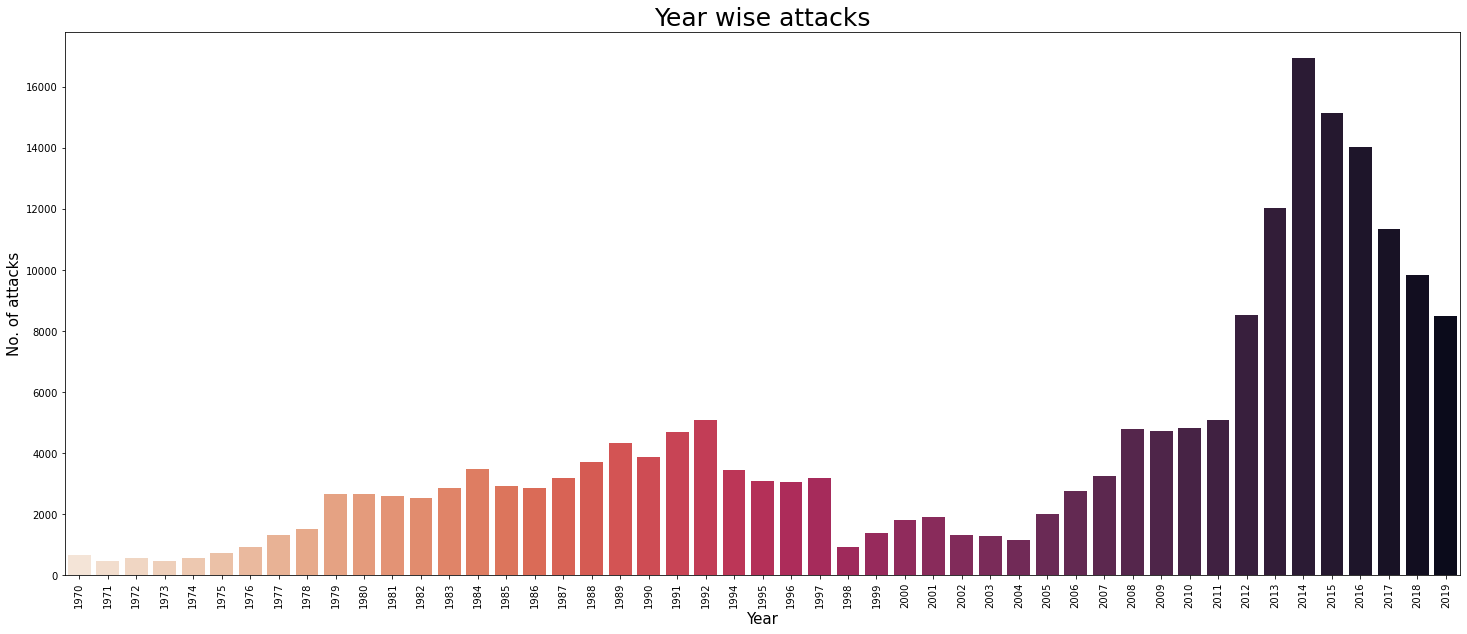
\includegraphics[height=4.2cm]{img/yearlytrend.png} 
\caption{No. of attacks each Year}
\label{fig:figure1}
\end{center}
\end{figure}

\section{Visualizing the target location of Kidnappers}
The kidnapping and hijacking type of terror from our dataset has been picked up and analysis is performed on those attacks. Figure \ref{fig:figure2} shows the origin and target locations (destinations) of the Kidnappers and Hijackers. 
The actual origin and the capital of destination countries have been marked. Looking at the map, it can be seen that most origin of kidnapping/hijacking attacks are the most from Southwest Asian and Central European countries. The destination of the kidnappers/hijackers is near the Caribbean, Western Asia and some isolated places.

\begin{figure} [h]
\begin{center}
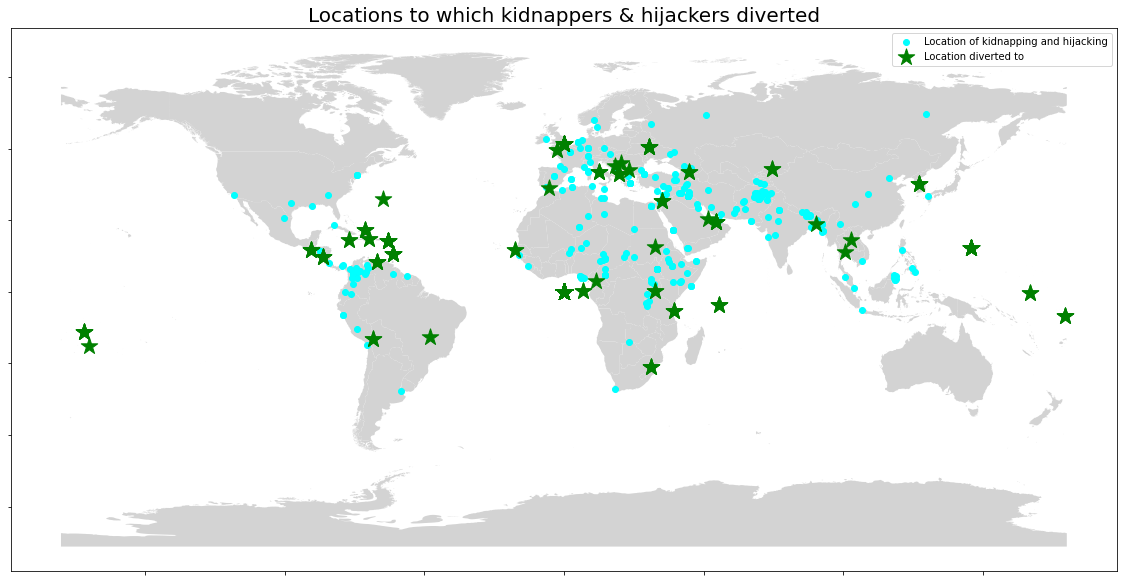
\includegraphics[height=7cm]{img/kidnaplocations.png} 
\caption{Hijacking/Kidnapping source and destination}
\label{fig:figure2}
\end{center}
\end{figure}


\section{Economic and Social Influence}
Terrorism has affected countries all over the world with major or minor losses. Terrorism has economic, psychological, and social consequences for any country exposed to terrorist events. The economic damage for countries with more than 1 million dollars of property loss can be seen in Figure \ref{fig:figure3}

\begin{figure} [h]
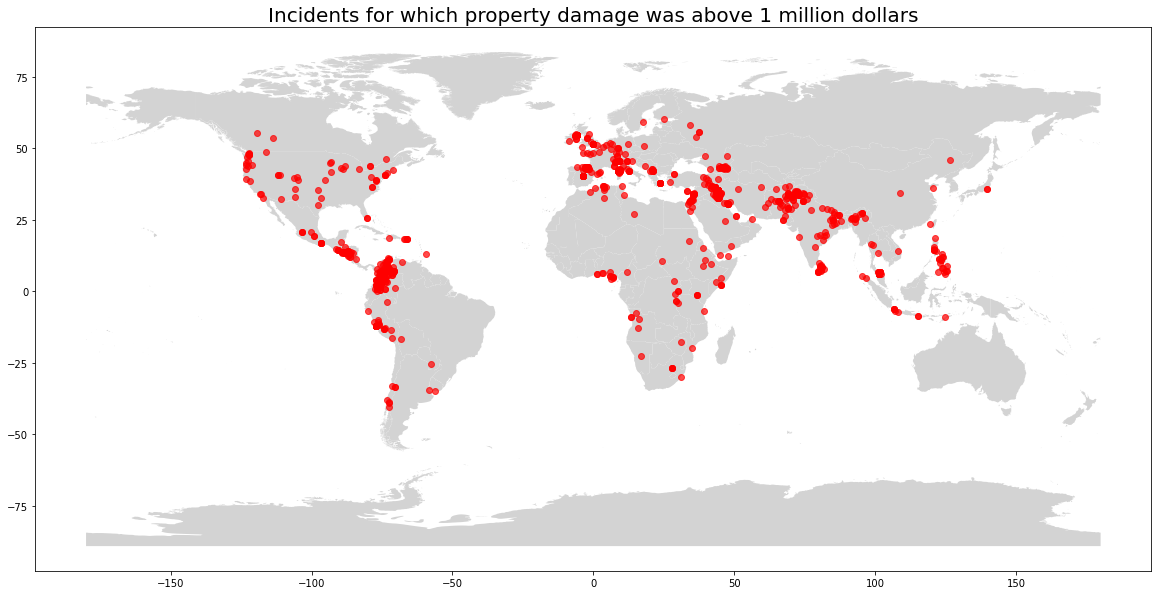
\includegraphics[height=7cm]{img/attackdamage.png} 
\caption{Map of countries with Property damage more than 1 million dollars}
\label{fig:figure3}
\end{figure}

To analyse psychological and social effects of terrorism on target country we relate terrorism with country wise Happiness ratio yearly. Support for this analysis can be found in the report of Turkey, 2017. \cite{turkey2017}
Continuing this analysis with our dataset, we use a World happiness dataset for years 2015 to 2019 and find a correlation between the number of terror attacks and happiness score of the country. On a scale of score of 1 being the least happy, the countries with higher terror attacks on the left of the threshold has a happiness score lower than the countries with lesser terror attacks on the right of the threshold. Thus, as terror attacks decrease the happiness score of the countries increases.
This analysis proves how terrorism has a social effect as well. See Figure \ref{fig:figure4}
\begin{figure} [h]
\begin{center}
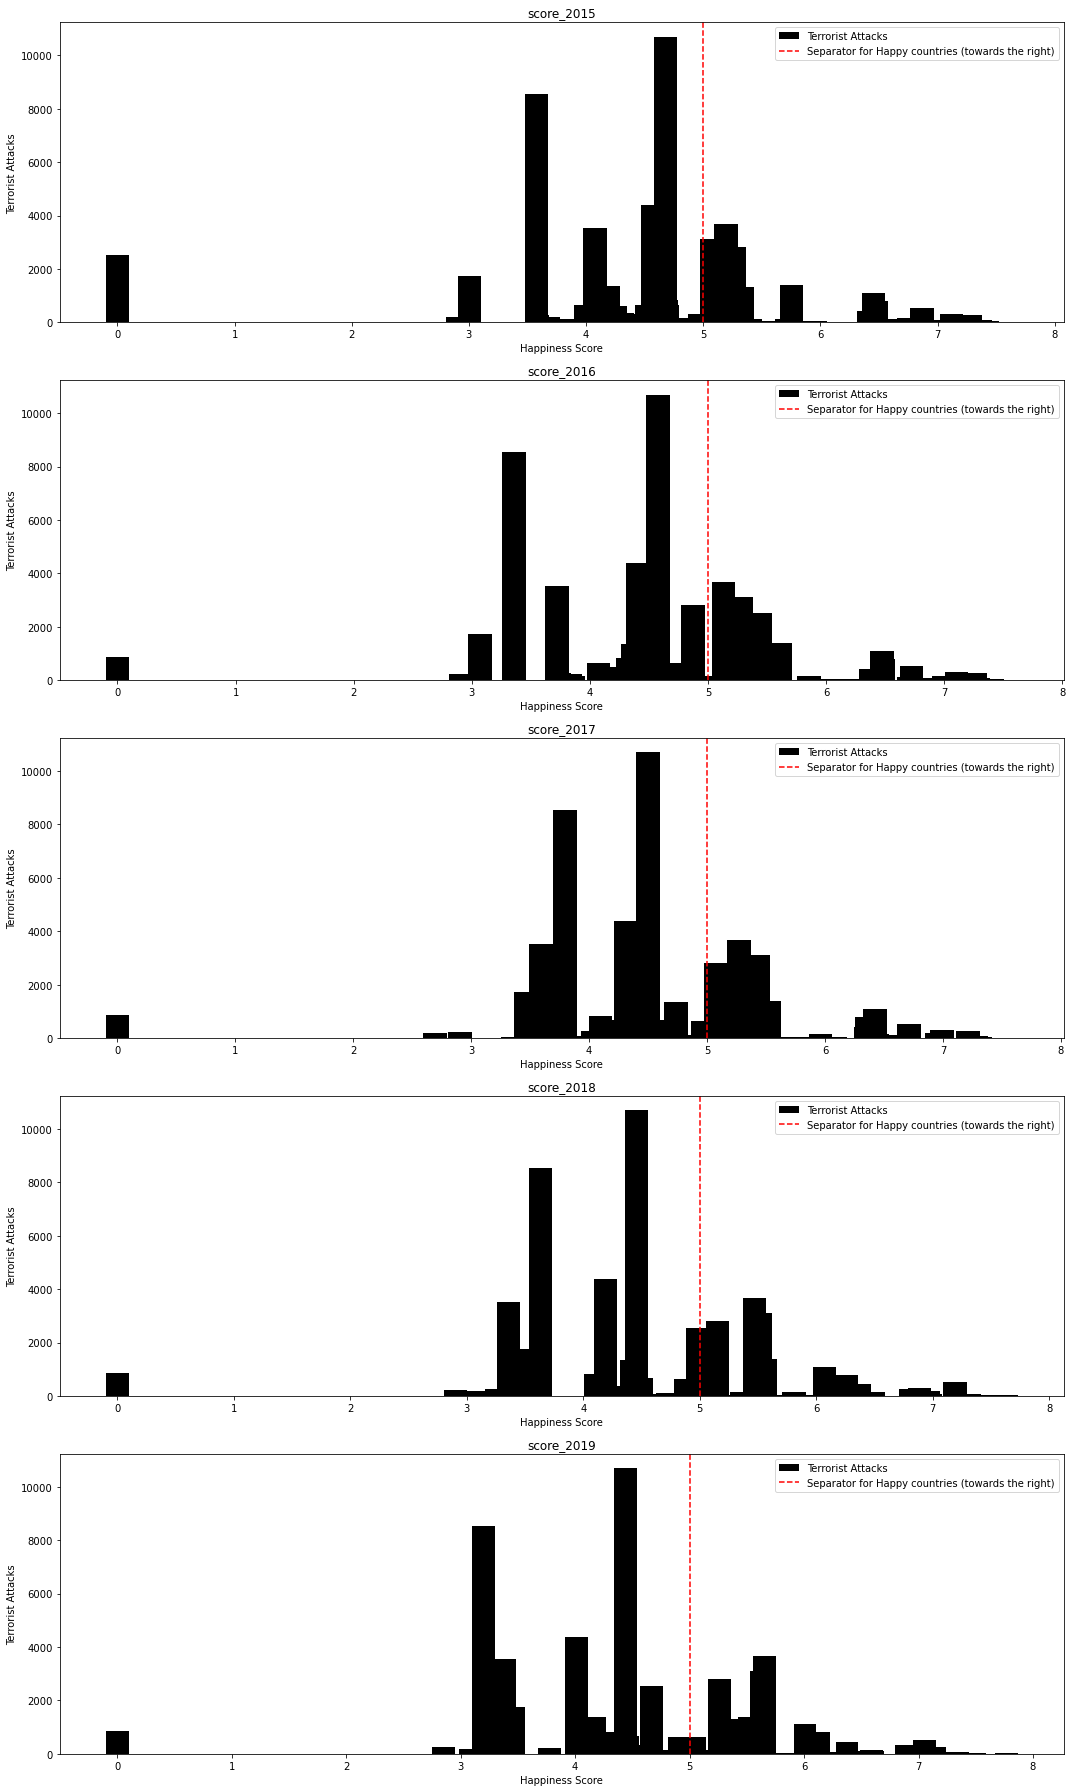
\includegraphics[width=10cm,height=10cm]{img/happinessscore.png} 
\caption{Are there lesser Terrorist attacks in Happier countries}
\label{fig:figure4}
\end{center}
\end{figure}

\section{Feature Importance and Predictions}
Using ExtraTreesClassifier for finding important features in our dataset. See Figure \ref{fig:figure5}
\begin{figure} [h]
\begin{center}
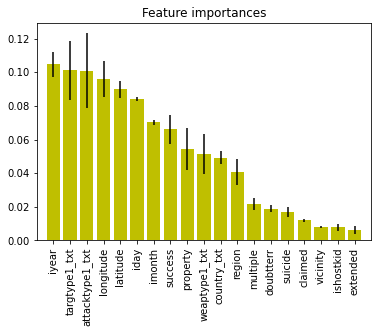
\includegraphics[height=5cm]{img/importantfeatures.png} 
\caption{Feature Importance}
\label{fig:figure5}
\end{center}
\end{figure}
\\We use 4 different classifiers to get the prediction accuracy of our model.\\
RandomForestClassifier gives 75\% accuracy\\
DummyClassifier gives 66\% accuracy\\
AdaBoostClassifier gives 77\% accuracy. Thus the best accuracy of all.\\
GradientBoostingClassifier gives 76\% accuracy
\section{Clustering}
Performing clustering on the dataset based on a few important features, clusters are formed in a way that it shadows the 12 regions in our dataset. 
The Similarity between cluster and region labels came up to 84.65 \%. See Figure \ref{fig:figure6}
\begin{figure} [h]
\begin{center}
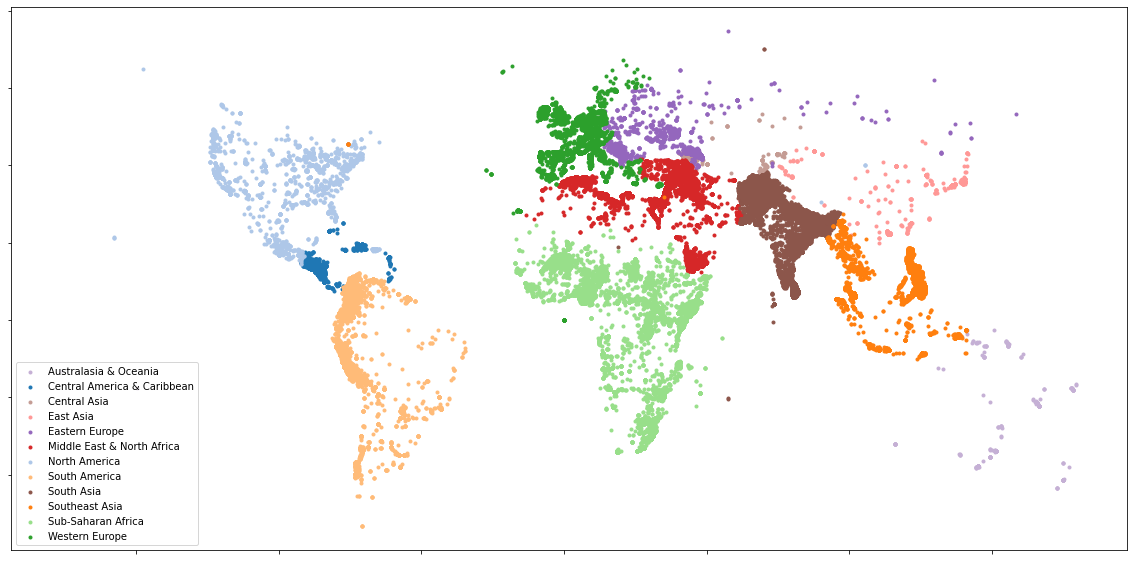
\includegraphics[height=7cm]{img/clustered.png} 
\caption{Clustered data}
\label{fig:figure6}
\end{center}
\end{figure}
\section{Conclusions and Future Scope:}
The act of terrorism causes major economic loss but along with also comes social, psychological loss. Similar to Happiness relativity with terrorism, other factors like political stability, economic status can also be tampered. Thus, an in depth understanding of effects of terrorism can be performed.


{
\small
\bibliography{sample}
}


%%%%%%%%%%%%%%%%%%%%%%%%%%%%%%%%%%%%%%%%%%%%%%%%%%%%%%%%%%%%

\end{document}